\section{V-model}

%Lyd - blackboks - nodeark
%
%Mic - lydfil - algoritme
%
%adc - lagring  Fourier - filter - spektogram - symbolbehandling
%
%S/h - Kvantisering  Passende fil
%
%
%
%
%V model og test specifikationer.
%På blackbox niveau - Test musik ind og nodeark ud.
%
%Lydfill - test musik ind lydfill ud.
%
%Algorithme - test lydfill ind - nodeark ud.
%
%
%
%Mikrofon - Test??
%
%adc - Test??
%
%S/h - test??
%
%kvantisering - test? 

The V-model is a simple multiple-phase model used to describe phases in the development process. 
The name V-model comes from V, that represents the different phases.
The first phase is description of the system and decomposition to smaller and more specific units.
Along with this phase a list of test specifications are created, starting from the smallest unit, and working up to the system as a hole.
Later on the these test will be conducted.
\\\\
\begin{figure}
\centering
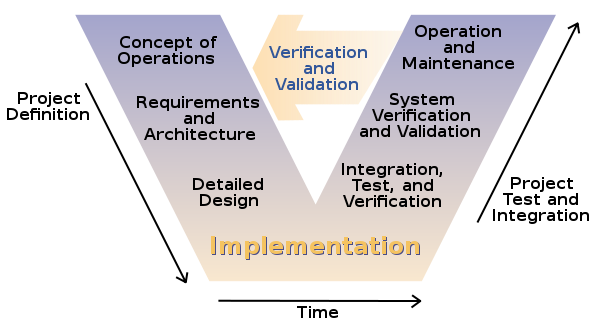
\includegraphics[scale=0.5]{figures/20170215_V-model_image.png}
\caption{Illustration of the V-model. \cite{V-modelwiki}}\\ \chr{Wiki link}
\end{figure}
The left side of the V, is decomposition of the problem, and the right side is the creation and integration and test of system.
In the synthesis section, the left part of the V-model is described, and hence the next step in the V-model is the creation of the test specifications for the different parts.
\chr{https://www.tutorialspoint.com/sdlc/sdlc_v_model.htm}
\subsection{Test specification / validation}
The V-model will be tested from the bottom up, starting with the smallest components (a unit). This validation phase is called the Unit testing. The test should checks each of the "units" individually and verify, that they are working according to expectations. \\\\
Next up the coherence of the system is tested, and finally the system it self as a single unit is tested. 
\\\\

\textbf{The  units in the model are as follows }
\begin{itemize}
	\item Microphone
	\item Sample and hold
	\item Quantization
	\item Sound file creation
	\item Fourier transformation
	\item Filter
	\item Spectrogram
	\item Note sheet creation
\end{itemize}


\subsubsection{Unit test of the Fourier transformation}
This test will be done by comparing the Fourier algorithm used, with a pre-existence algorithm from matlab or python.
By feeding the algorithms the same data set and comparing the output int. 
In addition to this, the algorithm will be tested on data with an expected result like a simple sinusoidal.
\subsubsection{Unit test on the choice of filter}
The filter will be tested on data with a high signal to noise ratio with noise expected to find in a normal use situation added on.
\subsubsection{Unit test of spectrogram}
As with verification of the Fourier transform, the spectrogram algorithm, will be tested against a pre- algorithm, on the same data set.
The algorithm will then be tested on a fixed data set with a known output.
By doing so, the output of the algorithm can hence be compared.
\subsubsection{Unit test of note sheet creation}
This test will be done by creating a spektrogram from a known note sheet, and trying to recreate the note sheet.
\chr{Evt. give dette en under element der beskriver mere specifikt hvordan spektrogrammet kreeres }
\chr{Note, not all of the components will be tested  as they are outside of the scope of the project - Afgrænsinger her ved beskrivelse af testende?? (Aka. her)}
\subsubsection{Integration validation}
The next step is to test the units as they are integrated into a single system.
This test is done by taking the output of the previous and feeding it into the next step of the algorithm. 
This is a minor step in creating the final product.
This product 
simple data 
\\\\
The music used for testing the algorithm will be simple melodies comtaining one note at a time (no chords) from one instrument at a time. This will allow insight into the methods used without complicating the recognition of notes by blending together different instruments and different sound frequencies.\\\\

\subsubsection{System test of the final product}
The final design, will be tested by giving the final system a recording with a known result and comparing the difference between the products result and the know result. The design can be further tested to see if all the wanted characteristics of the system comply to the wanted criteria of the system.


